% The Slide Definitions
%document
\documentclass[10pt]{beamer}
%theme
\usetheme{metropolis}
% packages
\usepackage{color}
\usepackage{listings}
\usepackage[ngerman]{babel}
\usepackage[utf8]{inputenc}
\usepackage{multicol}


% color definitions
\definecolor{mygreen}{rgb}{0,0.6,0}
\definecolor{mygray}{rgb}{0.5,0.5,0.5}
\definecolor{mymauve}{rgb}{0.58,0,0.82}

\lstset{
    backgroundcolor=\color{white},
    % choose the background color;
    % you must add \usepackage{color} or \usepackage{xcolor}
    basicstyle=\footnotesize\ttfamily,
    % the size of the fonts that are used for the code
    breakatwhitespace=false,
    % sets if automatic breaks should only happen at whitespace
    breaklines=true,                 % sets automatic line breaking
    captionpos=b,                    % sets the caption-position to bottom
    commentstyle=\color{mygreen},    % comment style
    % deletekeywords={...},
    % if you want to delete keywords from the given language
    extendedchars=true,
    % lets you use non-ASCII characters;
    % for 8-bits encodings only, does not work with UTF-8
    frame=single,                    % adds a frame around the code
    keepspaces=true,
    % keeps spaces in text,
    % useful for keeping indentation of code
    % (possibly needs columns=flexible)
    keywordstyle=\color{blue},       % keyword style
    % morekeywords={*,...},
    % if you want to add more keywords to the set
    numbers=left,
    % where to put the line-numbers; possible values are (none, left, right)
    numbersep=5pt,
    % how far the line-numbers are from the code
    numberstyle=\tiny\color{mygray},
    % the style that is used for the line-numbers
    rulecolor=\color{black},
    % if not set, the frame-color may be changed on line-breaks
    % within not-black text (e.g. comments (green here))
    stepnumber=1,
    % the step between two line-numbers.
    % If it's 1, each line will be numbered
    stringstyle=\color{mymauve},     % string literal style
    tabsize=4,                       % sets default tabsize to 4 spaces
    % show the filename of files included with \lstinputlisting;
    % also try caption instead of title
    language = Python,
	showspaces = false,
	showtabs = false,
	showstringspaces = false,
	escapechar = ,
}

\def\ContinueLineNumber{\lstset{firstnumber=last}}
\def\StartLineAt#1{\lstset{firstnumber=#1}}
\let\numberLineAt\StartLineAt



\newcommand{\codeline}[1]{
	\alert{\texttt{#1}}
}


% Author and Course information
% This Document contains the information about this course.

% Authors of the slides
\author{Claas de Boer, Tilman Hinnerichs}

% Name of the Course
\institute{Python-Grundlagen}

% Fancy Logo 
\titlegraphic{\hfill
\includegraphics[height=1.25cm]{../images/fsr_logo_cropped}}

% Custom Bindings
% \newcommand{\codeline}[1]{
%	\alert{\texttt{#1}}
%}


% Presentation title
\title{Modularisierung 2.0}

\date{\today}


\begin{document}

\maketitle

\section{Rückblick: Einbinden von Externen Bibliotheken}

\begin{frame}[fragile]{Vokabeln}
Auslagern von Code in nach Verantwortlichkeiten sortierte Module und Packages ermöglicht es eine übersichtliche Code Base aufzubauen.
\begin{itemize}
\item Modul $:=$ Python Datei \texttt{.py}
\item Package $:=$ \glqq Ordner \grqq von Modulen
\end{itemize}
\end{frame}

\begin{frame}[fragile]{Importieren eines Moduls}
    Zum Importieren eines Moduls/Package kann das \texttt{import} statement verwendet werden.
    \begin{lstlisting}
# Import des gesamten Inhalts eines Moduls/PKG
# **mit** dem Namespace des importierten Moduls
import random               # -> aufruf: random.randint()
import random as rnd        # -> aufruf: rnd.randint()

# Import des gesamten Inhalts eines Moduls/PKG
# **in** den Namespace des importierenden Moduls
from random import *        # -> aufruf: randint()

# Import einer einzelnen Funktion
# **in** den Namespace des importierenden Moduls
from random import randint  # -> aufruf: randint()
    \end{lstlisting}
\end{frame}

\begin{frame}[fragile]{Import Hilfen}

\begin{lstlisting}
import random

# Der Klassiker: help()
help(random)

# Liste alle importierten Variablen, Funktionen, und Klassen auf
dir(random)

# Gib den Speicherort des importierten Moduls aus
print(random.__file__)
\end{lstlisting}
\end{frame}

\begin{frame}[fragile]{Import Pitfalls}
Module \texttt{example.py}
\begin{lstlisting}
CONSTANT = 1

# Code der ausgeführt wird, wenn example.py ausgeführt wird
print("Hallo Mama, ich bin in einer Präsentation!")
\end{lstlisting}

\begin{lstlisting}
>>> import example
>>> Hallo Mama!
>>>
\end{lstlisting}
Wie können wir es vermeiden Code beim Import auszuführen?
\end{frame}

\begin{frame}[fragile]{Boilerplate Code}
Module \texttt{example.py}
\begin{lstlisting}
CONSTANT = 1

# Code der nur ausgeführt wird,
# wenn example.py direkt ausgeführt wird
if __name__ == "__main__":
    print("Hallo Mama, ich bin in einer Präsentation!")
\end{lstlisting}

\begin{lstlisting}
>>> import example
>>>
\end{lstlisting}
    Das in \texttt{example.py} enthaltene \texttt{print}-Statement wird nur ausgeführt, wenn \texttt{example.py} direkt ausgeführt wird.
\end{frame}

\begin{frame}[fragile]{Ein eigenes Package}
    \begin{center}
    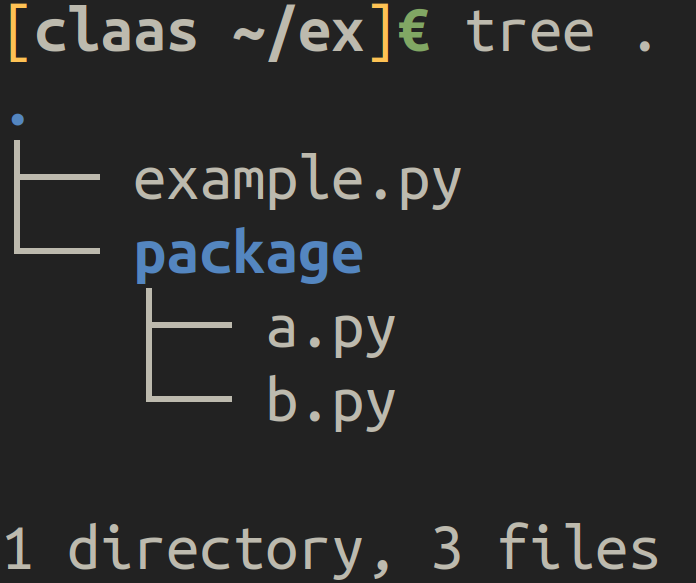
\includegraphics[height=.4\textheight]{Package.png}
    \end{center}
    In \texttt{example.py}:
    \begin{lstlisting}
# Import modul a aus package 'package'
import package.a

# Import modul b aus package 'package'
import package.b
\end{lstlisting}
\end{frame}

\begin{frame}[fragile]{Tipps}
    \begin{itemize}
        \item Importiere nur so viel wie nötig (vermeidet Überdeckungen im Namespace)
        \item Importiere nur von tieferen Hierarchie Leveln
        \item Vermeide zyklische Imports (A importiert B, B importiert A)
    \end{itemize}
\end{frame}

\begin{frame}[fragile]{Aufgaben}
    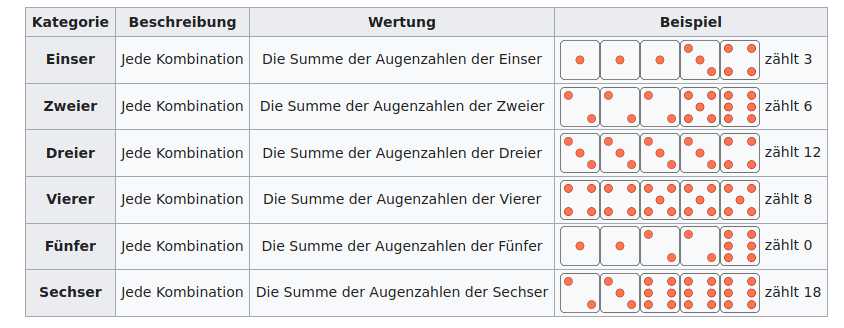
\includegraphics[width=\textwidth]{Kniffel_Tabelle_1.png}

    \begin{enumerate}
        \item Erweitere die Klasse des Würfelspielers, sodass dieser 5 Würfel besitzt (siehe voherige Sessions).
        \item Implementiere eine Scoring Funktion, die, ausgehend von 5 Resultaten (Liste) und einer Kategorie, den Wert der Resultate berechnet. Werden die Bedingungen der Kategorie nicht erfüllt, ist der Wurf 0 Punkte wert.
    \end{enumerate}
    \href{https://de.wikipedia.org/wiki/Kniffel}{Wikipedia: Kniffel}
\end{frame}

\begin{frame}[fragile]{Aufgaben}
    \begin{center}
        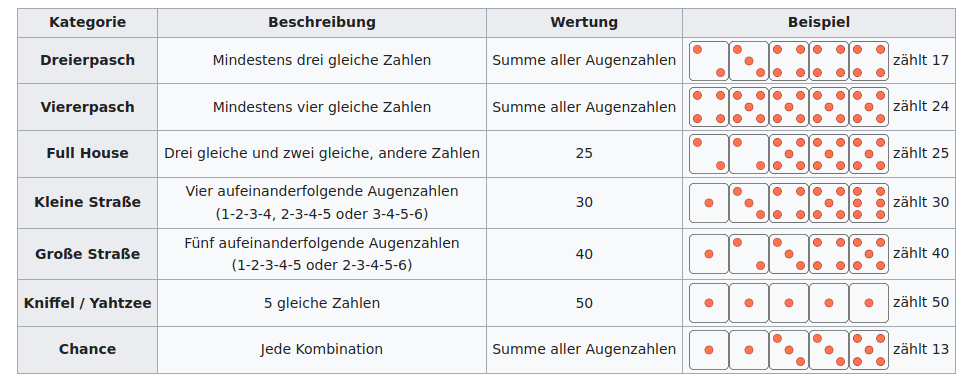
\includegraphics[width=.9\textwidth]{Kniffel_Tabelle_2.png}
    \end{center}
    \begin{enumerate}
        \item Ergänze die Kategorien um den Dreierpasch, den Viererpasch, das Full House, die Kleine Straße, die Große Straße, Kniffel sowie Chance.
        \item \textbf{Bonus}: Implementiere eine Funktion, die für einen Wurf den größtmöglichen Score sowie den Namen der dazugehörigen Kategorie ausgibt.
    \end{enumerate}
    Tipp: Vielleicht hilft dir \texttt{collections.Counter}
\end{frame}

\end{document}
